%%%%%%%%%%%%%%%%%%%%%%%%%%%%%%%%%%%%%%%%%%%%%%%
%% Introduction aux Systèmes d'exploitation  %%
%%   * Historique                            %%
%%   * Principes fondamentaux                %%
%%   * Grandes classes de systèmes           %%
%%%%%%%%%%%%%%%%%%%%%%%%%%%%%%%%%%%%%%%%%%%%%%%

\title{Le système UNIX}
\subtitle{Presentation du système UNIX}

\author{Yves \textsc{Stadler}}\institute{Codasystem, UPV-M}

\date{\today}



\begin{document}


%%
% Page de Titre
%%
\begin{frame}
\titlepage
\end{frame}


\section{Objectif du chapitre}
%%
% Présentation générale du cours
%%
\begin{frame}{Objectifs}
\begin{alertblock}{Nous allons voir}
\begin{itemize}
\item Le système de gestion de fichier d'UNIX
\item Les bases du langages BASH
\end{itemize}
\end{alertblock}

\begin{block}{Notions abordés dans ce module}
\begin{itemize}
\item L'interface CLI (Command Line Interface)
\item Fichiers (types, droits, etc...)
\item Commandes simples et paramétrées
\item Programmes de commandes, scripts
\item Interaction avec le système d’exploitation
\end{itemize}
\end{block}
\end{frame}

\section{Historique et évolution}
\subsection{Historique}
\begin{frame}{Historique et évolution}
\begin{block}{Naissance}
\begin{itemize}
\item UNIX est né en 1969, et conçu par Ken Thomson aux laboratoires Bell d'AT\&T.
\item Deux familles : BSD (Berkley Software Distribution) et SystemV (AT\&T).
\end{itemize}

\end{block}

\begin{block}{Évolution}
\begin{itemize}
\item Standardisation POSX $\leftarrow$ convergence des deux familles.
\item Développement des IHM $\leftarrow$ apparition des deux variantes : MOTIF (IBM) et OPEN LOOK (Sun et AT\&T)
\end{itemize}

\end{block}

\begin{block}{Distribution}
\begin{itemize}
\item Versions commercialles (Solaris et AIX)
\item Domaine public avec Linux
\end{itemize}
\end{block}

\end{frame}

\subsection{Caractéristiques}
\begin{frame}{Caractéristiques}
\begin{block}{Généralités}
\begin{itemize}
\item Multi-utilisateurs
\item Multi-tâches
\item Universel
\item SGF (Système de gestion de fichier) arborescent
\item Processus hiérarchisés
\end{itemize}
\end{block}
\end{frame}


\subsection{Universalité}
\begin{frame}{Universalité}
\begin{alertblock}{Portabilité}
L'objectif d'UNIX est d'avoir une conception portable (i.e. compatible et adaptable)
\end{alertblock}

\begin{block}{Composantes}
\begin{itemize}
\item Noyau
\item Interface homme-machine
\item Outils
\end{itemize}
\end{block}
\end{frame}

\subsection{Gestion des processus}
\begin{frame}{Gestion des processus}
\begin{alertblock}{Définition}
Activité associée a l'exécution d'un programme.
\end{alertblock}

\begin{block}{Gestion}

\begin{itemize}
\item Interface assurée par une bibliothèque de fonctions primitives du langage C
\item Création de processus : fork()
\item Synchronisation et communications avec d'autres processus : wait(), pipe(), ...
\item Relation hiérarchisée des processus : père-fils.
\end{itemize}
\end{block}
\end{frame}



%%%%%%%%%%%%%%%%%%%%%%%%%%%%
\section{Système de gestion de fichiers}
\subsection{La structure arborescente}
\begin{frame}{Système de gestion de fichiers}
\begin{block}{La structure arborescente}
\begin{itemize}
\item Structure arborescente = répertoire (directory)
\item Les noeuds sont des répertoires
\item Les feuilles sont des fichiers
\item La racine est le point de départ de la structure (en anglais : root)
\end{itemize}
\end{block}

\begin{block}{title}
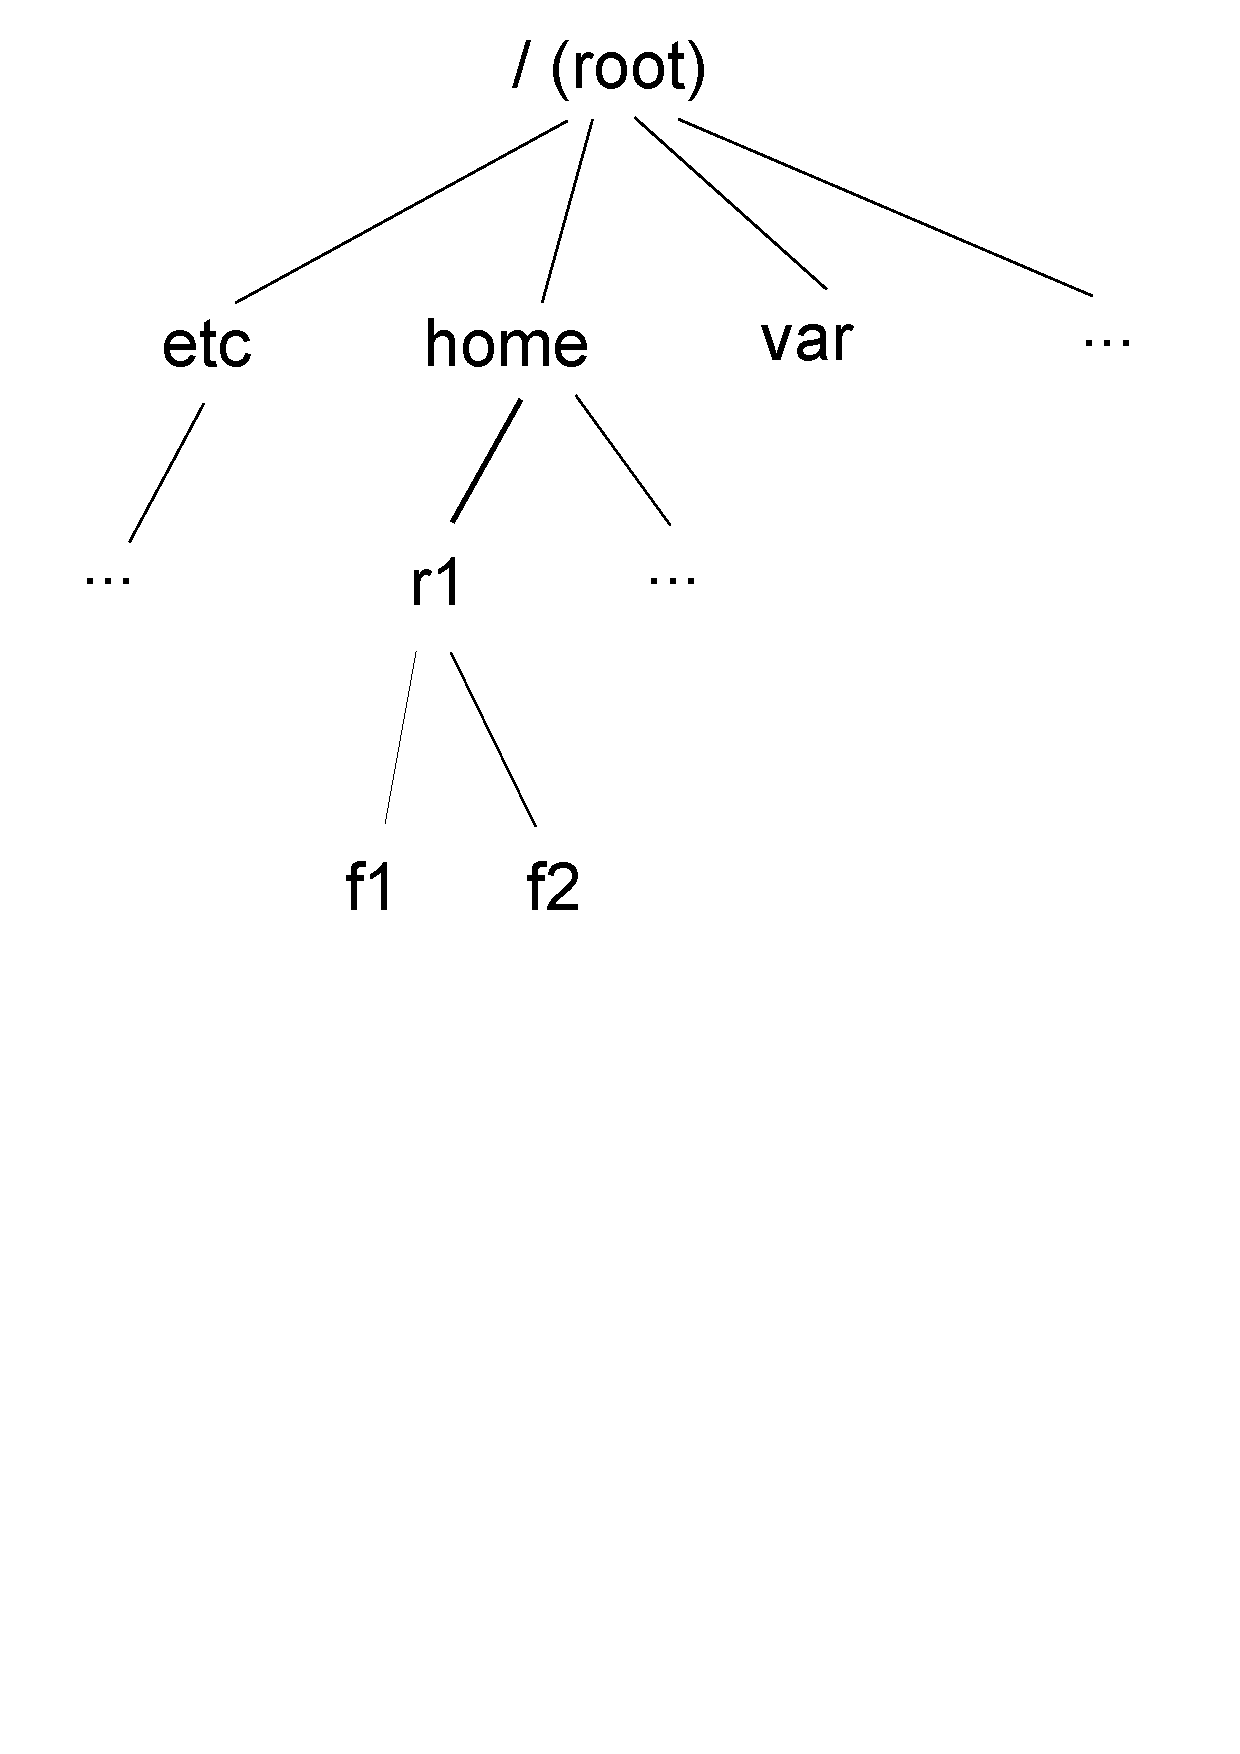
\includegraphics[width=0.5\textwidth]{CH02-IntroductionUnix/images/arbo.pdf}
\end{block}

\end{frame}

\begin{frame}{Système de gestion de fichiers}
\begin{block}{Exemples de répertoires}
\begin{itemize}
\item dev : concerne les périphériques
\item bin : contient des exécutables
\item etc : fichiers pour les utilisateurs systèmes
\item usr : répertoire des programmes utilisateurs, \url{/usr/bin} commandes du systèmes
\end{itemize}
\end{block}

\end{frame}


\subsection{Accès}
\begin{frame}{Accès à l'arborescence}
\begin{block}{Deux types d'accès}
Accéder à l'arborescence, c'est désigner la référence (fichier ou répertoire) que l'on souhaite utiliser :
\begin{itemize}
\item par un chemin
\item par un lien
\end{itemize}
\end{block}
\end{frame}

\begin{frame}{Accès à l'arborescence}
\begin{block}{Chemin arborescent}
Deux manières :
\begin{itemize}
\item par un chemin absolu
\item par un chemin relatif
\end{itemize}
\end{block}

\begin{block}{Exemple avec le fichier f1}
\begin{itemize}
\item Absolu : \url{/home/r1/f1}
\item Si l'on se trouve dans le répertoire \url{/home} : \url{r1/f1}
\end{itemize}
\end{block}
\end{frame}

\begin{frame}{Accès à l'arborescence}
\begin{block}{Lien}
On peut créer des liens désignant un fichier, ou un répertoire (commande ln)
\begin{itemize}
\item Ils apparaissent comme un fichier, ou un répertoire (transparence)
\item Ils ont les mêmes droits
\item Ils accèdent aux même emplacement physique
\end{itemize}
\end{block}

\begin{alertblock}{Remarques}
Modifier le contenu d'un lien modifie le contenu de l'original, mais détruire un lien ne détruit pas l'original.
\end{alertblock}
\end{frame}


\subsection{Types de fichiers}
\begin{frame}{Types de fichiers}
\begin{block}{Trois types}
\begin{itemize}
\item Ordinaire (suite d'octets stucturés selon un format)
\item Répertoire (contient les références à d'autres fichiers, et leurs attributs : droits, position sur le disque, ...)
\item Spécial  (associé à un périphérique)
\end{itemize}
\end{block}
\end{frame}

\begin{frame}{Protection des fichiers}
\begin{block}{Type de protection}
\begin{itemize}
\item Contre la lecture
\item Contre la modification
\item Contre l'exécution
\end{itemize}
\end{block}

\begin{block}{Interdire qui?}
\begin{itemize}
\item  Moi
\item  Mon groupe
\item Les autres
\end{itemize}
\end{block}

\end{frame}

\begin{frame}{Protection des fichiers}

\begin{block}{Champs (attribut de fichier)}
\begin{center}
\begin{tabular}{|c|c|c|}
\hline
U & G & O\\
\hline
r x w & r x w & r x w \\
\hline
\end{tabular}
\end{center}
\end{block}

\begin{block}{Légende}
\begin{itemize}
\item  User Group Others
\item  Read Write eXecute
\item  Absence de droit : -
\end{itemize}
\end{block}

\end{frame}


\begin{frame}{Protection des fichiers}
\begin{block}{Change mode}
\texttt{chmod 777 [fich1] [fich2]}\\
\texttt{chmod u+rxw [fich1] [fich2]}
\end{block}

\begin{block}{Correspondance}
\begin{center}
\begin{tabular}{|c|c|c|}
\hline
U & G & O\\
\hline
1 1 1 = 7 & 0 0 1 = 1 & 0 0 0 = 0 \\
\hline
r x w & r x w & r x w \\
\hline
\end{tabular}
\end{center}
\end{block}

\end{frame}

\section{Langage de commande}

\begin{frame}{Langage de commande}
\begin{alertblock}{CLI}
Ou Command Line Interface, c'est ce qui permet à l'utilisateur par le moyen de mots clés, d'agir directement avec le système.
\end{alertblock}

\begin{block}{Interpréteur de commande}
Appellé aussi terminal il constitu l'interface entre l'utilisateur et la CLI.
\begin{itemize}
\item Il permet de se loguer
\item Il permet de saisir des commandes (entrée standard)
\item Il permet d'afficher les résultats (sortie standard)
\item Il permet de voir les erreurs (sortie d'erreur standard)
\end{itemize}
\end{block}
\end{frame}

\begin{frame}{Commandes de base}
\begin{block}{Juste après le login}
\begin{itemize}
\item \texttt{whoami} : me dit qui je suis (ex: ystadler)
\item \texttt{id} : mon numéro d'utilisateur (ex: uid=500)
\item \texttt{groups} : à quel groupe j'appartiens (ex: profs)
\item \texttt{pwd} : dans quel répertoire je suis
\end{itemize}
\end{block}

\begin{block}{Les répertoires}
\begin{itemize}
\item \texttt{cd [directory]} : change directory
\item \texttt{cd ..} : revenir au répertoire parent
\item \texttt{cd .} : changer pour le répertoire courant
\item \textasciitilde : home, répertoire de l'utilisateur en cours
\end{itemize}

\end{block}
\end{frame}


\begin{frame}{Commandes de bases}
\begin{block}{List}
\begin{itemize}
\item \texttt{ls [directory]} : donne la liste des répertoires et fichiers
\item \texttt{ls -a} : liste tous les fichiers/reps
\item \texttt{ls -l} : affiche une liste de fichiers/reps avec leurs attributs
\end{itemize}
\end{block}

\begin{block}{ls -l}
\texttt{drxw---r-x 2 root root 47  Jun 10 2008 Desktop/ \\
drxw---r-x 2 root root 12  Jun 10 2008 F1/ \\
-rxw---r-x 2 root root 121 Jun 10 2008 f1 \\
-rxw---r-x 2 root root 113 Jun 10 2008 f2 \\
-rxw---r-x 2 root root 114 Jun 10 2008 f3
}
\end{block}
\end{frame}


\begin{frame}{Commandes de base}
\begin{block}{Lecture, écriture}
\begin{itemize}
\item \texttt{cat [fichier]} : liste le contenu d'un fichier sur l'entrée standard
\item \texttt{cat} : on  lit sur stdin et on écrit sur stdout
\item \texttt{cat > fichier} : écrit dans un fichier
\item CTRL-D = End Of File (EOF)
\end{itemize}

 
\end{block}

\begin{block}{Création, destruction}
\begin{itemize}
\item \texttt{mkdir directory} : créer un répertoire
\item \texttt{touch file} : créer un fichier vide (ou modifie le last accès d'un fichier existant
\item \texttt{rmdir directory} : supprimer un répertoire
\item \texttt{rm file} : supprimer un fichier
\end{itemize}
\end{block}
\end{frame}

\begin{frame}{Commandes de bases}
\begin{block}{Les options}
\begin{itemize}
\item \texttt{rm -f file} : supprimer un fichier sans confirmation
\item \texttt{rm -r}: suppression récursive
\item \texttt{rm -rf}: suppression récursive sans confirmation
\item \texttt{mkdir -p ../../directory} : créer un répertoire et ses parents si nécessaire.
\end{itemize}
\end{block}

\begin{block}{Les options longues}
\begin{itemize}
\item \texttt{rm --help} : affiche l'aide
\item \texttt{./configure --prefix=/usr/bin}
\end{itemize}
\end{block}
\end{frame}

\begin{frame}{Find et grep}
\begin{block}{Find}
\texttt{find [path] [expression]}\\
expression := (EXPR) | !EXPR | -not EXPR | EXPR1 -a(nd) EXPR2 | EXPR1 -o(r) EXPR2\\

\end{block}

\begin{block}{grep}
\texttt{grep [-iv] terme [fichier]} : rechreche dans les fichiers le terme (-i cas insensitive, -v negation)
\end{block}

\begin{alertblock}{Méta-caractères}
\begin{itemize}
\item \textasciicircum début de ligne
\item \url{$} fin de ligne
%$ syntax coloration
\end{itemize}
\end{alertblock}
\end{frame}

\subsection{Les scripts}
\begin{frame}{Les scripts}
\begin{block}{Définition}
Liste de commande que l'interpréteur de commande va interpréter. C'est un programme.
\end{block}

\begin{block}{Le Sha bang}
\url{\#!/bin/bash} : il indique le type d'interpréteur que l'on va utiliser pour exécuter le programme.\\
\url{\#!/usr/bin/python}
\end{block}

\begin{alertblock}{Remarque}
Un script doit être exécutable pour pouvoir se lancer de cette manière : ./script ; Sinon il faut appeller l'interpréteur soit même : bash script
\end{alertblock}
\end{frame}

\subsection{Les variables}
\begin{frame}{Variables}
\begin{block}{Les variables}
\begin{itemize}
\item Affectation : a=valeur
\item Lecture : \$a
\end{itemize}
\end{block}

\begin{block}{Variable d'environnement}
\begin{itemize}
\item Variables utiles pour les processus systèmes
\item On les listes avec : \texttt{env}
\item {\$}PWD : répertoire en cours
\item {\$}PATH : chemins d'accès des commandes exécutables directement.
\item {\$}SHELL : shell utilisé par défaut.	
\end{itemize}
\end{block}
\end{frame}

\subsection{Les tests}
\begin{frame}{Tests}
\begin{block}{If... then... else.. fi}
if (test); then (command); else (command); fi\\
if\\
(test)\\
then\\
(command)\\
else\\
 (command)\\
fi
\end{block}

\begin{block}{Exemple}
if\\
 \verb![! {\$}a -eq 2 \verb!]!\\
then\\
echo "Hello"\\
else\\
 echo "World"\\
fi
\end{block}

\end{frame}

\begin{frame}{Les tests}
\begin{block}{Faire un test}
\begin{itemize}
\item \verb![ expression ]!
\item -a fichier : vrai si le fichier existe
\item -s fichier : vrai si le fichier existe, et a une taille non nulle.
\item -d fichier : vrai si le fichier est un répertoire
\item -r fichier : vrai si le fichier est exécutable (idem pour -w -x)
\item -z chaine : vrai si la chaine est nulle
\item -n chaîne : vrai si la longueur de la chaîne est non-nulle. 
\end{itemize}
\end{block}
\end{frame}

\begin{frame}{Les tests}
\begin{block}{Faire un test}
\begin{itemize}
\item chaîne\_1 == chaîne\_2
    Vrai si les deux chaînes sont égales. Le symbole = peut servir à remplacer == 
\item chaîne\_1 != chaîne\_2
    Vrai si les deux chaînes sont différentes. 
\item chaîne\_1 $<$ chaîne\_2
    Vrai si chaîne\_1 se trouve avant chaîne\_2 dans l'ordre lexicographique de la localisation en cours. 
\item chaîne\_1 $>$ chaîne\_2
    Vrai si chaîne\_1 se trouve après chaîne\_2 dans l'ordre lexicographique de la localisation en cours. 
\item arg1 OP arg2
    OP est l'un des opérateurs suivants -eq, -ne, -lt, -le, -gt, ou -ge.
\end{itemize}
\end{block}
\end{frame}

\subsection{Les boucles}
\begin{frame}{Boucles}
\begin{block}{For in do done}
for (variable) in (liste de valeur)\\
do\\
(commands)\\
done
\end{block}


\begin{block}{while do done}
while/until (test)\\
do\\
(commands)\\
done
\end{block}
\end{frame}

\begin{frame}{Case et select}
\begin{block}{case}
case (variable) in\\
valeur) (commands);;\\
valeur2) (commands);;\\
*) (commands);;\\
esac
\end{block}

\begin{block}{select}
select (variable) in (liste)\\
Créer un menu numéroté pour chaque entrée de la liste\\
La selection de l'utilisateur est stocké dans la variable.
\end{block}
\end{frame}

\subsection{Variables utiles}
\begin{frame}{Variables utiles}
\begin{block}{Quelques variables symboliques}
\begin{itemize}
\item {\$}0 : nom de la commande invoquée
\item {\$}n : valeur du nième argument (1-9)
\item la commande shift permet de décaler les arguments (2 dans 1, 3 dans 2, etc...)
\item {\$}\# : le nombre d'arguments utilisés lors de l'appel du script
\end{itemize}
\end{block}
\end{frame}


\begin{frame}{Merci}
\begin{center}
La suite en TD.
\end{center}
\end{frame}
%%
% Fin du document
%%




\end{document}
